
\section{Lösungsversprechen von Vue}
Vue wird zunächst als ein progressiver Framework bezeichnet.
Das bedeutet, dass es sich an die Bedürfnisse des Entwicklers anpasst.Während andere Frameworks eine vollständige Übernahme einer Technologie durch einen Entwickler oder ein Team erfordern und oft möchten, dass eine existierende Anwendung neu geschrieben wird, weil bestimmte Konventionen erforderlich sind. Vue landet zunächst mit einem einfachen Skript-Tag in einer Anwendung und kann mit den Anforderungen wachsen, von einer kleinen Web-Komponente bis hin zur Verwaltung der gesamten Ansichtsebene.
Es ist nicht notwendig, über Webpack, Babel, npm oder ähnliches Bescheid zu wissen, um mit Vue zu beginnen. HTML , CSS und Grundlagen von JavaScript reichen aus, um mit Vue anzufangen.

Der Sprung von einer reinen HTML- und CSS-basierten Website zu einer anspruchsvollen Webanwendung ist sehr einfach gehalten und kann im Laufe des Entwicklungsprozesses erlernt werden.
Dies ist ein starkes Verkaufsargument, insbesondere im aktuellen Ökosystem der JavaScript-Frontend-Frameworks und -Bibliotheken, das Neueinsteigern und auch erfahrenen Entwicklern das Gefühl gibt, im Ozean der Möglichkeiten und Wahlmöglichkeiten verloren zu gehen.
Das Ziel von Vue ist es, mit minimalem Vorkenntnisse vernünftige Web-Applikationen erstellen zu können.


{\let\clearpage\relax \chapter{Vue.js}}
% \chapter{Vue.js}
\label{sec:grundlagen}

Vue ist ein skalierbares JavaScript Framework zum Aufbau von Benutzeroberflächen. Im Gegensatz zu anderen Frameworks ist Vue von Grund auf so konzipiert, dass es schrittweise anpassbar ist. Die Kernbibliothek ist nur auf die Ansichtsebene (View) ausgerichtet und lässt sich leicht in andere Bibliotheken oder bestehende Projekte integrieren. In Kombination mit modernen Tools und zusätzlichen Bibliotheken, ist Vue  in der Lage, anspruchsvolle Single-Page-Applikationen zu betreiben \cite{Vue019:Intro:Online}.

\section[]{Haupt Merkmale }
\label{sec:Einführung}
% \subsection{VueJS}
% \label{sec:VueJS}


Vue ist zusammen mit React und Angular eines der beliebtesten Frameworks in der Webentwicklungslandschaft. Folgende Merkmale zeichnen das Vue-Framework aus:
\begin{labeling}{Components:::::}
	\item [Components:] Vue-Komponenten erweitern grundlegende \gls{HTML}-Elemente, um wiederverwendbaren Code zu kapseln. Das Vue-Komponenten-System ist eine Abstraktion, die die Erstellung großer Anwendungen aus kleinen, in sich geschlossenen und oft wiederverwendbaren Komponenten ermöglicht.
	\item [Templates:] Vue.js verwendet eine HTML/\gls{CSS}-basierte Template-Syntax. Vue kompiliert  die Vorlagen (Templates) in virtuelle \gls{DOM}-Renderfunktionen. In Kombination mit dem Reaktivitätssystem ist Vue in der Lage, intelligent die minimale Anzahl von Komponenten, die aktualisiert werden müssen, zu ermitteln. Dies minimiert die Anzahl von DOM-Manipulationen bei der Zustandsänderung der Applikation.
	\item [Reaktivität:] Vue verfügt über ein Reaktivitätssystem, welches reine JavaScript-Objekte verwendet und das Rendering optimiert. Jede Komponente behält während des Renderns den Überblick über ihre reaktiven Abhängigkeiten. Das ermöglicht dem System intelligent und optimal die Komponenten neu zu rendern.
  \item [Integrierbarkeit:] Es ist sehr einfach, Vue in bestehende Projekte zu integrieren oder Bibliotheken von Drittanbietern zu Vue hinzuzufügen. Alle JavaScript-Bibliotheken, die ES6+ verwenden, können innerhalb von Vue verwendet werden. Zum Beispiel Bootstrap, Material Design, ThreeJS, Web Sensors API usw.  Vue bietet auch die Möglichkeit, TypeScript anstelle von JavaScript zu verwenden.
	
\end{labeling}
\cite{VueGuide:Online}

\section{Vue im Vergleich zu Angular und React}
\label{sec:Vue im Vergleich zu Angular und React}
 Vue wurde von Evan You entwickelt, als er bei Google an AngularJS (Angular 1.0)-Anwendungen arbeitete.Vue übernahm einen Teil der Angular-Templating-Syntax aus, entfernte jedoch den komplexen Stack, den Angular erforderte. Dadurch wurde es sehr leistungsfähig. Das neue Angular (Angular 2.0) löste auch viele der AngularJS-Probleme, jedoch auf sehr unterschiedliche Weise, und erfordert TypeScript, das nicht alle Entwickler gerne verwenden (oder lernen wollen).

Vue hat viele gute Ideen von React übernommen, vor allem das virtuelle DOM.  Aber Vue implementiert es mit einer Art automatischer Abhängigkeitsverwaltung, die nachverfolgt, welche Komponenten von einer Änderung des Zustands betroffen sind, so dass nur diese Komponenten neu gerendert werden, wenn sich die Zustands-Eigenschaft ändert. In React hingegen wird bei einer Änderung eines Teils des Zustandes, der Auswirkungen auf eine Komponente hat, diese Komponente neu gerendert, und damit werden auch alle zugehörigen Kinder-Komponente neu gerendert. Dies ist ein Vorteil für Vue in Bezug auf die Benutzerfreundlichkeit und die Leistungssteigerung \cite{VueComparision:Online}.

\begin{table}[H]
	\centering
	\caption{Vue vs React vs Angular}
	\label{tab:table_VueJS}
	\begin{tabular}{{p{3cm}|p{3cm}|p{3cm}|p{3cm}}}
    \toprule
    Kriterium & 
\includegraphics[width=0.05\textwidth]{Bilder/img/vue.png} & 
\includegraphics[width=0.05\textwidth]{Bilder/img/react.png} & 
\includegraphics[width=0.05\textwidth]{Bilder/img/angular.png}\\
     & Vue & React & Angular\\
    \midrule
    Fokus & Nutzbarkeit & Flexibilität & TypeScript \\
    Komplexität & Niedrig & Mittel & Hoch \\
    Größe & 80 KB & 100 KB  & 500+ KB\\
    Veröffentlichung & 2014 & 2013  & 2010 \\
    Entwickelt von & Evan You & Facebook & Google \\
    Sprache & JavaScript & JavaScript & TypeScript\\
    Model & virtuelle DOM & virtuelle DOM & \gls{MVC}\\
    Unterstütz von & Open Source & Facebook  & Google \\
    Aktuellste Version & 2.6.11 & 16.13.1 & 9.1.11\\
		\bottomrule
	\end{tabular}
\end{table}
\cite{ComparisonVue:Online}


\section{Struktur eines Vue.js Projekts}
\label{sec:Struktur eines Vue.js Projekts}
Vue hat eine sehr intuitive Projektstruktur. Zusätzlich zum Kern des Frameworks enthält es eine Menge Utilities, die die Frontend-Entwicklung mit Vue sehr angenehm machen.
Wie meisten JavaScript Projekte wird für Vue-Entwicklung NodeJS verwendet. Vue stellt die Kernbibliothek und die Zusatz Utilities über \texttt{\textbf{\gls{npm}} (node package manager)} zur Verfügung.

\paragraph{NodeJS} ist eine JavaScript-Laufzeitumgebung, die auf der V8-JavaScript-Engine von Chrome basiert. Sie ermöglicht die Ausführung von JavaScript-Code außerhalb eines Webbrowsers. NodeJS ermöglicht es Entwicklern, JavaScript zum Schreiben von Kommandozeilen-Tools und für die serverseitige Ausführung von Skripten zu verwenden, um dynamische Webseiteninhalte zu erzeugen, bevor die Seite an den Webbrowser des Benutzers gesendet wird. NodeJS unterstützt die Vereinheitlichung der Web-Anwendungsentwicklung um eine einzige Programmiersprache herum, anstatt verschiedene Sprachen für server- und clientseitige Skripte zu verwenden \cite{NodeJS:Online}.

\paragraph{npm (node package manager)} ist die größte Software-Registry der Welt. Open-Source-Entwickler aus allen Kontinenten nutzen npm, um Pakete gemeinsam zu nutzen und auf sie zuzugreifen, und viele Organisationen nutzen npm auch zur Verwaltung der privaten Entwicklung \cite{NPM:Online}.

\paragraph*{Vue-CLI:} Vue bietet eine offizielle CLI(Command Line Interface) für das schnelle Einrichten anspruchsvoller einseitiger Anwendungen. Es bietet einen umfassenden Build-Setup für einen modernen Frontend-Workflow. Es dauert nur wenige Minuten, um mit Hot-Reload, Lint-on-Save und Produktions-Builds in Betrieb zu gehen.

\paragraph{Installiation}
Die Installation der erforderlichen Pakete wird mit NodeJS und npm durchgeführt. Folgende Befehle müssen ausgeführt werden um ein Basis Vue Anwendung zu erstellen:
\begin{itemize}
  \item Die Vue-CLI global installieren:
  \begin{lstlisting}[language=bash]
    npm install -g @vue/cli
  \end{lstlisting}
  \item Die Vue-\gls{CLI} wird verwendet um einen neuen Vue-Projekt zu erstellen.
  \begin{lstlisting}[language=bash]
    vue create beispiel_vue_app
  \end{lstlisting}
  Dadurch wird eine CLI geöffnet, in der die gewünschte Konfiguration für ein Vue-Projekt eingestellt werden kann.
  \item Um den Entwicklungsserver zu starten, wird der folgende Befehl ausgeführt:
  \begin{lstlisting}[language=bash]
    npm run serve
  \end{lstlisting}
  \item Um einen Production-Build für die App zu erzeugen, wird folgender Befehl ausgeführt:
  \begin{lstlisting}[language=bash]
    npm run build
  \end{lstlisting} 
\end{itemize} 

Ein typisches Vue-Projekt mit Vue-Router und Vuex hat die folgende Struktur:

\begin{table}[H]
	\centering
	\caption{Struktur des Projektordners}
	\label{tab:table_VueJS}
	\begin{tabular}{{p{4cm}p{9cm}}}
		\toprule
		Dateien/Ordner  & Beschreibung\\
		\midrule
    public/index.html & Dies ist die Haupt-App-Datei, die vom Browser geladen wird. 
    Die Datei enthält im Body nur ein einfaches HTML-Tag: \texttt{ \textcolor{red}{<div id=\enquote{app}> </div>}}. 
    Dies ist das Element, mit dem die Vue-Anwendung an das DOM angehängt wird. \\
    \hline
    src/main.js & Dies ist die JavaScript-Datei, die für die Konfiguration der Vue.js Anwendung verantwortlich ist. Es wird auch verwendet, um alle Pakete von Drittanbietern zu registrieren. \\
    \hline
    src/App.vue & Dies ist die Root-Komponente, die den HTML-Inhalt enthält, der dem Benutzer angezeigt wird. \\
    \hline
    /package.json & In dieser Datei speichert npm die Namen und Versionen des Pakets, das es installiert hat. \\
    \hline
    src/components/ & Dieser Ordner enthält die zusätzlichen Komponenten. \\
    \hline
		src/assets/ & Dieser Ordner wird verwendet, um statische Inhalte, wie Bilder zu speichern. \\
    \hline
		src/router/ & Der Ordner enthält die Implementierung von Vue-Router. \\
		\hline
		src/store/ & Der Ordner enthält die Implementierung von Vuex-Store. \\
    \bottomrule
	\end{tabular}
\end{table}

% \begin{lstlisting}[language=JavaScript, caption=package.json]
% {
%   "name": "vue_pwa",
%   "version": "0.1.0",
%   "scripts": {
%     "serve": "vue-cli-service serve",
%     "build": "vue-cli-service build",
%   },
%   "dependencies": {
%     "vue": "^2.6.11",
%     "vue-router": "^3.1.6",
%     "vuetify": "^2.2.11",
%     "vuex": "^3.1.3"
%   },
%   "devDependencies": {
%     "@vue/cli-plugin-router": "~4.3.0",
%     "@vue/cli-plugin-vuex": "~4.3.0",
%     "@vue/cli-service": "~4.3.0",
%   },
% }

% \end{lstlisting}
\section{Das Vue Instanz} Jede Vue-Anwendung beginnt mit der Erstellung einer neuen Vue-Instanz (Root Instance) mit der Vue-Funktion. Wenn eine Vue-Instanz erstellt wird, fügt sie dem Reaktivitätssystem von Vue alle in ihrem Datenobjekt(beschrieben in Tabelle \ref{tab:table_data}) gefundenen Eigenschaften hinzu.  Alle zu verwendende \texttt{Vue.js} internen Module und externen Plugins werden in der Datei \texttt{(main.js)} mit ES6(ECMAScript 2015) Import Syntax ('import') importiert. Die Abhängigkeiten sind als globale Parameter definiert und sind von allen Komponenten zugänglich.  
% Ein typischer VueJS Projekt hat eine Struktur wie im Abbildung \ref{fig:vue_projekt_struktur}. 
In der main.js Datei wird die Haupt-Vue-Komponente (\texttt{App.vue}) registriert. 
%Die Funktion der einzelnen Dateien in dem Projektordner sind in der Tabelle \ref{tab:table_VueJS} beschrieben.
\begin{lstlisting}[language=JavaScript, caption=main.js]
    import Vue from 'vue'
    import App from './App'
    import router from './router'

    // Root Instance
    new Vue({
        el: '#app',
        router,
        template: '<App/>',
        components: { App }
    })

\end{lstlisting}

\section{Vue Komponente}Das wichtigste Kriterium für die Auswahl dieses Frameworks \texttt{(Vue.js)} ist die Modularität der einzelnen Komponenten (beschrieben im Abschnitt \ref{sec:Einführung}). Die Komponenten sind eine der stärksten Eigenschaften von \texttt{Vue.js}. Sie ermöglichen, grundlegende HTML-Elemente zu erweitern, um wiederverwendbaren Code zu kapseln. Auf einer hohen Ebene sind Komponenten benutzerdefinierte Elemente, an die der \texttt{Vue.js} Compiler ein bestimmtes Verhalten anhängt \cite{Vue019:Intro:Online}. Jede Komponente wird in einer Datei mit \texttt{.vue} Erweiterung definiert. Die Definition enthält ein HTML basiertes Template, die die Gestaltung der Komponente festlegt und den JavaScript Code, das alle andere Funktionalitäten bzw. Verhalten der Komponente spezifiziert. Jede Komponente ist ebenfalls eine Vue-Instanz.

Üblicherweise wird eine Vue.js App in einem Baum aus verschachtelten Komponenten organisiert. Beispielsweise besteht sie aus Komponenten für einen Header, eine Seitenleiste und einen Inhaltsbereich, die jeweils andere Komponenten für Navigationslinks, Blog-Posts usw. enthalten. Die Komponenten Architektur vereinfacht solche Verschachteltelung.
\begin{figure}[H]
  \centering
  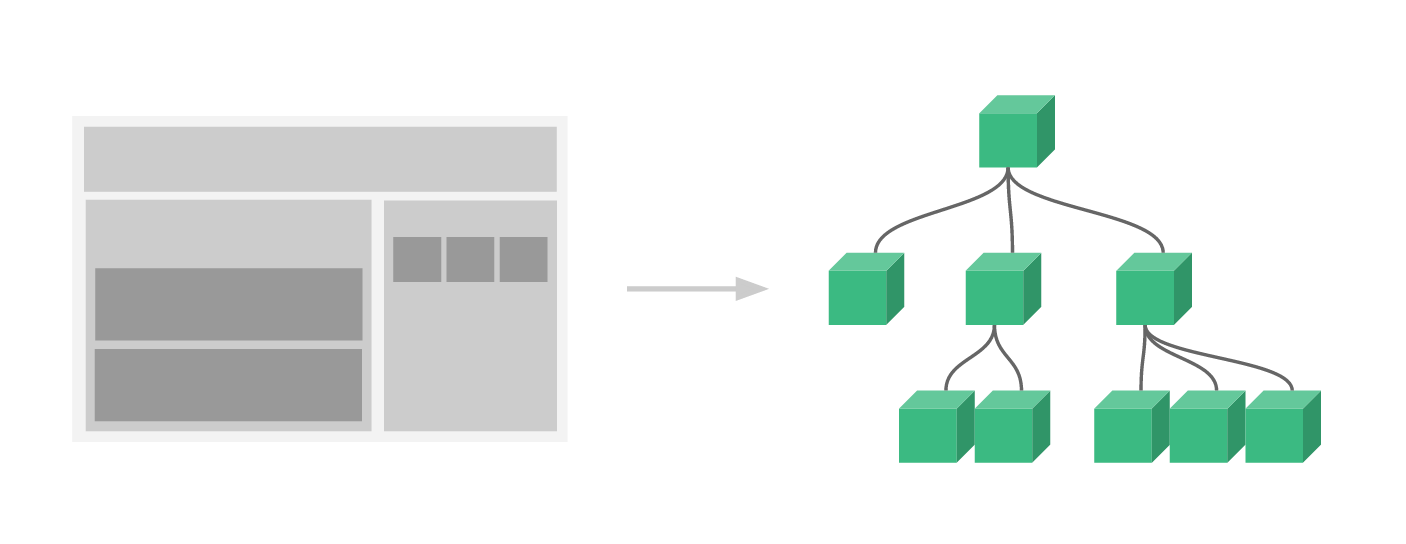
\includegraphics[width=0.6\textwidth]{Bilder/img/components.png}  
  \caption{ \textit{Organisation von Komponenten} \cite{VueComponents:Online}}%
\label{fig:Organisation von Komponenten}
\end{figure}

% Die grundlegende Struktur einer \texttt{Vue.js} Komponente ist im Listing \ref{lst:label} dargestellt. 

Das Template-Element beinhaltet das HTML-Template und das Script-Element beinhaltet den JavaScript-Teil der Komponente.
\begin{labeling}{Template-Element::}
	\item [Template-Element:] Die Gestaltung bzw. das Design der Benutzeroberfläche wird in deisem Element implementiert. Dafür wird Standard HTML und CSS Technik verwendet. Es können sowohl benutzerdefinierte HTML-Element als auch HTML-Elemente aus externen Plugins sehr einfach integriert werden. Die HTML-basierte Template-Syntax von Vue.js ermöglicht es, das gerenderte DOM deklarativ an die Daten der zugrunde liegenden Vue-Instanz zu binden. Alle Vue. js-Templates sind gültiges HTML.
	
	Die einfachste Form der Datenbindung ist die Textinterpolation unter Verwendung der \enquote{Mustache}-Syntax (doppelte geschweifte Klammern):
	\begin{lstlisting}[language=html,label={lst:label}, caption=Templateelement]
        <template>
            <div>
                <h1>Data: {{ beispielData }}</h1>
                <BeispielComponent/>
            </div>
        </template>    
        \end{lstlisting}
	\item [Script-Element:] Dieses Element beinhaltet die Implementierung der gewünschten Funktionalitäten der Komponente mit \texttt{VueJS} spezifischem Konstrukt. Weitere Komponenten können hier importiert und registriert werden. Diese stehen dann im Template-Element zur Verfügung, welches die Verschachtelung von Komponenten realisieren lässt.
	\begin{lstlisting}[language=JavaScript,label={lst:label}, caption=Skriptelement]
        
        <script>
          import BeispielComponent from 'components/BeispielComponent'
          export default {
            components: {
              BeispielComponent
            },
            props : [],
            data () {
              return {
                beispielData: 'Beispiel String'
              }
            },
            methods: {
                beispielFunction: function () { }
            },
            computed: {
            }
          }
        </script>
        
        \end{lstlisting}
\end{labeling}


Die wichtigsten Teile einer Komponente sind in der Tabelle \ref{tab:table_data} beschrieben.
\begin{table}[H]
	\centering
	\caption{Parameter zuständig für Datenmanipulation}
	\label{tab:table_data}
	\begin{tabular}{{p{1.7cm}p{4cm}p{8cm}}}
		\toprule
		Parameter & Typ & Beschreibung\\
        \midrule
        components &[key: string]: Object &Dies ist eine Liste von zu verwendenden benutzerdefinierten Komponenten. Die benutzerdefinierten bzw. externen Komponenten werden mit \texttt{\textcolor{purple}{import}} Befehl aus ES6 Spezifikation importiert.\\
		data & Object | Function & Dies ist ein JavaScript Objekt oder eine Funktion, die die Speicherung der notwendigen Attribute für die Komponente erlaubt. Innerhalb der Komponente kann auf das ursprüngliche Datenobjekt mit \texttt{\textcolor{purple}{this.data}} Direktive zugegriffen werden.\\
		props&Array<string> | Object & Dies ist eine Liste/Hash von Attributen, die zur Aufnahme von Daten aus der übergeordneten Komponente vorgesehen sind. Es hat eine einfache Array-basierte Syntax und eine alternative Objekt-basierte Syntax, die erweiterte Konfigurationen wie Typprüfungen, benutzerdefinierte Validierung und Standardwerte ermöglicht. \\
        methods&[key: string]: Function  & Dies ist eine Liste von Methoden, die die Realisierung verschiedener Funktionalitäten der Komponente erlauben.  Alle Methoden können innerhalb der Komponente als eine standard JavaScript Methode aufgerufen werden.\\
        computed&[key: string]: Function & Dies ist eine Liste von Methoden, die automatisch bei Änderung der reaktiven Abhängigkeiten aufgerufen wird. Die Attribute innerhalb dieser Parameter werden zwischengespeichert und nur bei reaktiven Abhängigkeitsänderungen neu berechnet. \\
		\bottomrule
	\end{tabular}
\end{table}


\section{Instanz-Lebenszyklus Hooks} Bei der Erstellung durchläuft jede Vue-Instanz eine Reihe von Initialisierungsschritten, z. B. muss sie die Datenbeobachtung einrichten, die Template kompilieren, die Instanz in das DOM einbinden und das DOM aktualisieren, wenn sich die Daten ändern. Parallel dazu werden auch Funktionen ausgeführt, die als Lifecycle-Hooks bezeichnet werden und den Benutzern die Möglichkeit geben, in bestimmten Phasen des Instanz-Lebenszyklus ihren eigenen Funktionen hinzuzufügen. Dies ermöglicht eine sehr präzise Steuerung des Verhaltens einzelner Komponenten.

Der \enquote{created} Hook kann beispielsweise zur Ausführung von Code nach der Erzeugung einer Instanz verwendet werden. Es gibt auch andere Hooks, die in verschiedenen Phasen des Lebenszyklus der Instanz aufgerufen werden, wie z.B. \enquote{mounted}, \enquote{updated} und \enquote{destroyed}. Die Abbildung \ref{fig:Organisation von Komponenten} illustriert die Details des kompletten Lifecycle-Hooks.

\begin{figure}[H]
  \centering
  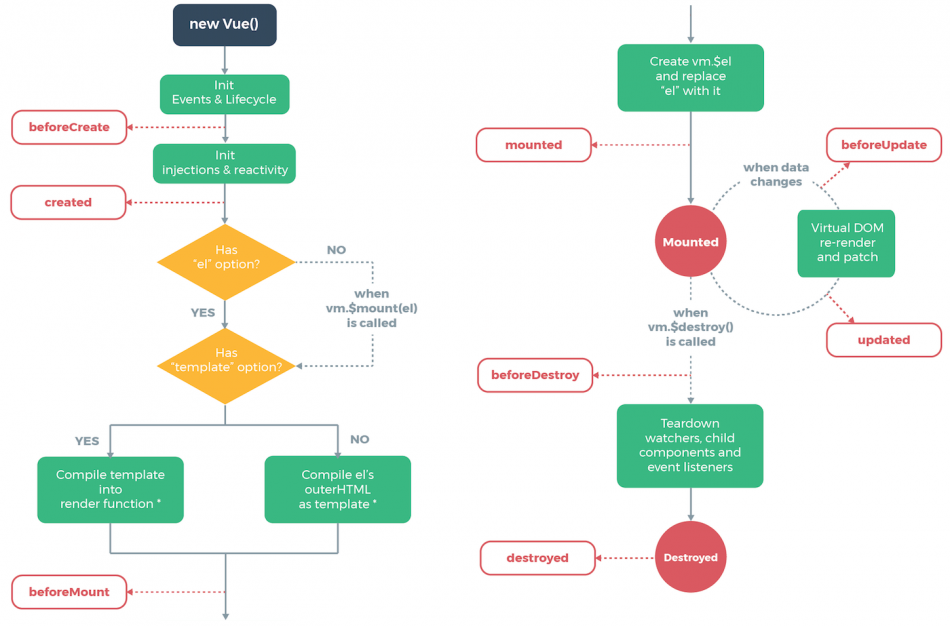
\includegraphics[width=1\textwidth]{Bilder/img/lifecycle_.png}  
  \caption{ \textit{Vue Instanz-Lifecycle Hooks} \cite{InstancVue:Online}}%
\label{fig:Organisation von Komponenten}
\end{figure}





% \begin{figure}[H]
% 	\centering
% 	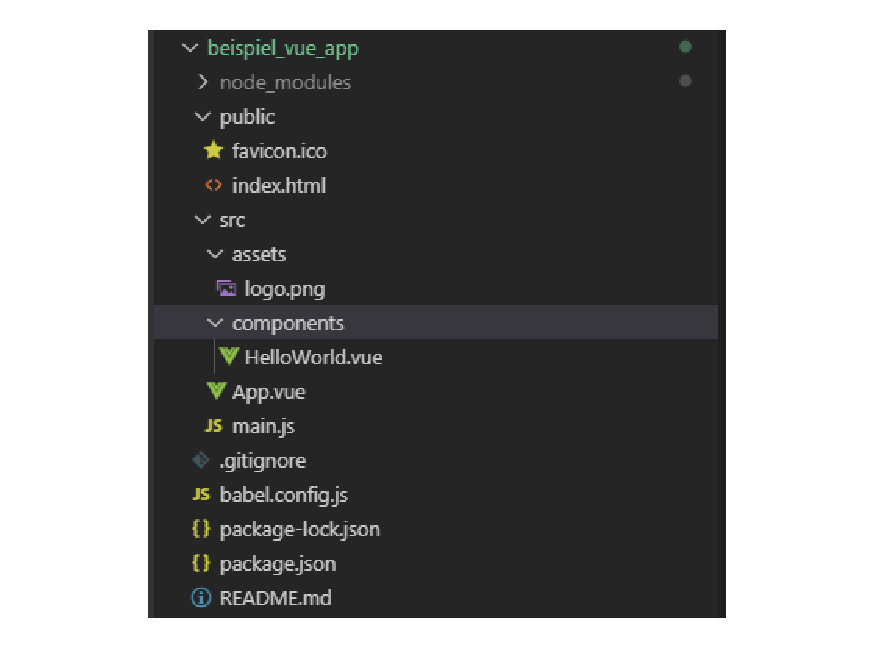
\includegraphics[width=1\textwidth]{img/vue_projekt_struktur.pdf}  
% 	\caption{ \textit{Vue.Js Projekt Struktur}}%
% \label{fig:vue_projekt_struktur}
% \end{figure}


\section{Vuex }
\label{sec:Vuex}
Vuex ist die offizielle Zustandsverwaltungsbibliothek für Vue. Ihre Aufgabe besteht darin, Daten zwischen den Komponenten einer Vue Anwendung auszutauschen.

Komponenten in einer Vue-Anwendung können ihren eigenen Zustand haben. Beispielsweise speichert ein Eingabefeld die darin eingegebenen Daten lokal. Komponenten können eine Eingabefeld sein oder eine ganze Seite. Es wird sehr aufwendig die Zustandsdaten zwischen verschachtelten Komponenten auszutauschen.

Vuex bietet einen zentralen Repository-Speicher(Vuex-Store) für den Zustand, und der Zustand kann durch den Aufruf von im Vuex-Store definierten Funktionen geändert werden.
Jede Komponente, die von einem bestimmten Teil des Zustands abhängt, greift auf diesen über einen getter Funktion auf dem Vuex-Store zu, wodurch Synchronisierung der Daten sichergestellt wird. Vuex-Store ist eine Art temporäre Datenbank für eine bestimmte Anwendungssitzung \cite{VueGuide:Online}.


\section{Vue Router }
\label{sec:Vue Router}

In einer Webanwendung ist ein Router der Teil, der die aktuell angezeigte Ansicht mit dem Inhalt der Browser-Adressleiste synchronisiert.

Ein Router wird benötigt, wenn \gls{URL}s mit den Ansichten in einer Anwendung synchronisiert werden müssen. Dies ist eine sehr häufige Notwendigkeit, und alle wichtigen modernen Frameworks erlauben inzwischen die Verwaltung des Routings.   Vue Router ist Teil der Vue Kern Bibliothek und übernimmt die Routenverwaltung in einer Vue-Anwendung \cite{VueGuide:Online}.

\newpage
{\let\clearpage\relax \chapter{Evaluation}}

Als Prototyp zum Testen der oben genannten Technologie wurde eine Einkaufsliste App entwickelt. Das Grundlayout wurde unter Verwendung von Standard-HTML und CSS entwickelt, und der Inhalt der Einkaufsliste wurde mit der Textinterpolations-Funktion von Vue implementiert. Jedes Element in der Einkaufsliste ist eine Vue-Komponente. Die entwickelte App verwendet die von Vue angebotene verschachtelte Komponentenarrhitektur. Vuex wird verwendet, um die Daten in der Einkaufsliste zu verwalten.
Der Quellcode der Prototyp-Anwendung, die mit dieser Technologie entwickelt wurde, ist in diesem Git-Repository zu finden: \url{https://git.efi.th-nuernberg.de/gitea/yadavaa81855/vue_pwa.git}

Es war insgesamt eine sehr angenehme Erfahrung, die App zu entwickeln. Wirklich gute Dokumentation und einfache Anwendbarkeit des Frameworks machen die Lernkurve ziemlich flach. Die Integration von Drittbibliotheken ist nicht kompliziert. Es war nicht notwendig, alles über das Framework zu lernen, um eine einfache App zu erstellen, und neue Funktionen können der App mit Hilfe dieses Frameworks leicht hinzugefügt werden.

\begin{table}[H]
	\centering
	\caption{Bewertung von VueJS anhand entwickelte Prototyp}
	\label{tab:table_VueJS}
	\begin{tabular}{{p{3cm}p{10cm}}}
		\toprule
		Kriterien  & Bewertung\\
		\midrule
		Lernkurve & In der Entwicklung überzeugt Vue.js durch die gute Erlernbarkeit der verschiedenen Konzepte, die aufeinander aufbauen.  \\
		\hline
    Modularität & Das Kern-Framework ist also sehr schlank und überschaubar und hat nur wenige Grundbausteine. Zusätzliche Funktionalitäten können mit Hilfe von Zusatzmodulen hinzugefügt werden \\
    \hline
    Skalierbarkeit & Es kann verwendet werden, um kleine Websites bis hin zu anspruchsvollen Webanwendungen zu erstellen. \\
    \hline
		Ökosystem & Vue.js verfügt über ein umfassendes Ökosystem mit Unterstützung für Bibliotheken und Plugins von Drittanbietern. \\
    \bottomrule
	\end{tabular}
\end{table}

 \chapter{Fazit}
Vue.js ist vielleicht nicht das am weitesten entwickelte Framework, aber es erfüllt manche Anforderungen vollkommen richtig. Erstens können sehr schnell und ohne großen Aufwand schöne Widgets und Anwendungen geschrieben werden. Die Lernkurve ist niedrig, das Belohnungsgefühl ist enorm hoch. Anfänger werden ihren Spaß mit Vue.js haben, vor allem weil alles so überschaubar ist.
Vue.js skaliert auch mit den Bedürfnissen des Teams und dem Wissensstand des Entwicklers und wird von der Entwickler-Community gut angenommen. 

Die Komponentenarchitektur von Vue.js hilft, die Anwendung so zu strukturieren, dass es einfach ist, durch die Teile der Anwendung zu navigieren, die von anderen Entwicklern entwickelt wurden. Die robusten \gls{API}s ermöglichten es, sich auf die Implementierung der Geschäftslogik zu konzentrieren, anstatt sich mit dem Framework zu befassen.

Vue.js verfügt über eine ausgezeichnete Online-Dokumentation mit vielen Beispielen.  Zusätzlich gibt es einen Vue.js Style Guide, der Best Practices zeigt, ein Vue.js-Kochbuch, das häufig verwendete Muster beschreibt, und eine Übersicht über zusätzliche Bibliotheken und Vue.js-Erweiterungen.